
\documentclass[sigconf]{acmart}

\usepackage{todonotes}
\usepackage{hyperref}

\usepackage{endfloat}
\renewcommand{\efloatseparator}{\mbox{}} % no new page between figures

\usepackage{booktabs} % For formal tables

\settopmatter{printacmref=false} % Removes citation information below abstract
\renewcommand\footnotetextcopyrightpermission[1]{} % removes footnote with conference information in first column
\pagestyle{plain} % removes running headers

\begin{document}
\title{Mapping Police Killing of Citizens in the United States}

\author{Jeramy Townsley}
\orcid{1234-5678-9012}
\affiliation{%
  \institution{IUPUI}
  \streetaddress{425 University Ave}
  \city{Indianapolis} 
  \state{Indiana} 
  \postcode{46202}
}
\email{jtownsle@indiana.edu}


\begin{abstract}
With the rise of camera phones that allows citizens to videotape law enforcement brutality against citizens, and the ability to immediately make those videos public through social media, there has been an increased awareness of police killings of citizens.  With this new data there have been a number of systematic attempts to document these events, from journalists, to academics, to activists, since there is no credible government database documenting this problem. These events can be mapped at the county level with the open source software QGIS.  Further, demographic and economic data gathered by the Census at the county level can be collected and tested against the police-killings to determine if a regression model can be used to describe a pattern among these variables. 
\end{abstract}

\keywords{i523, hid347, police brutality, multivariate regression, gis mapping, census, zero-inflated models}

\maketitle

\section{Introduction}


\begin{figure}
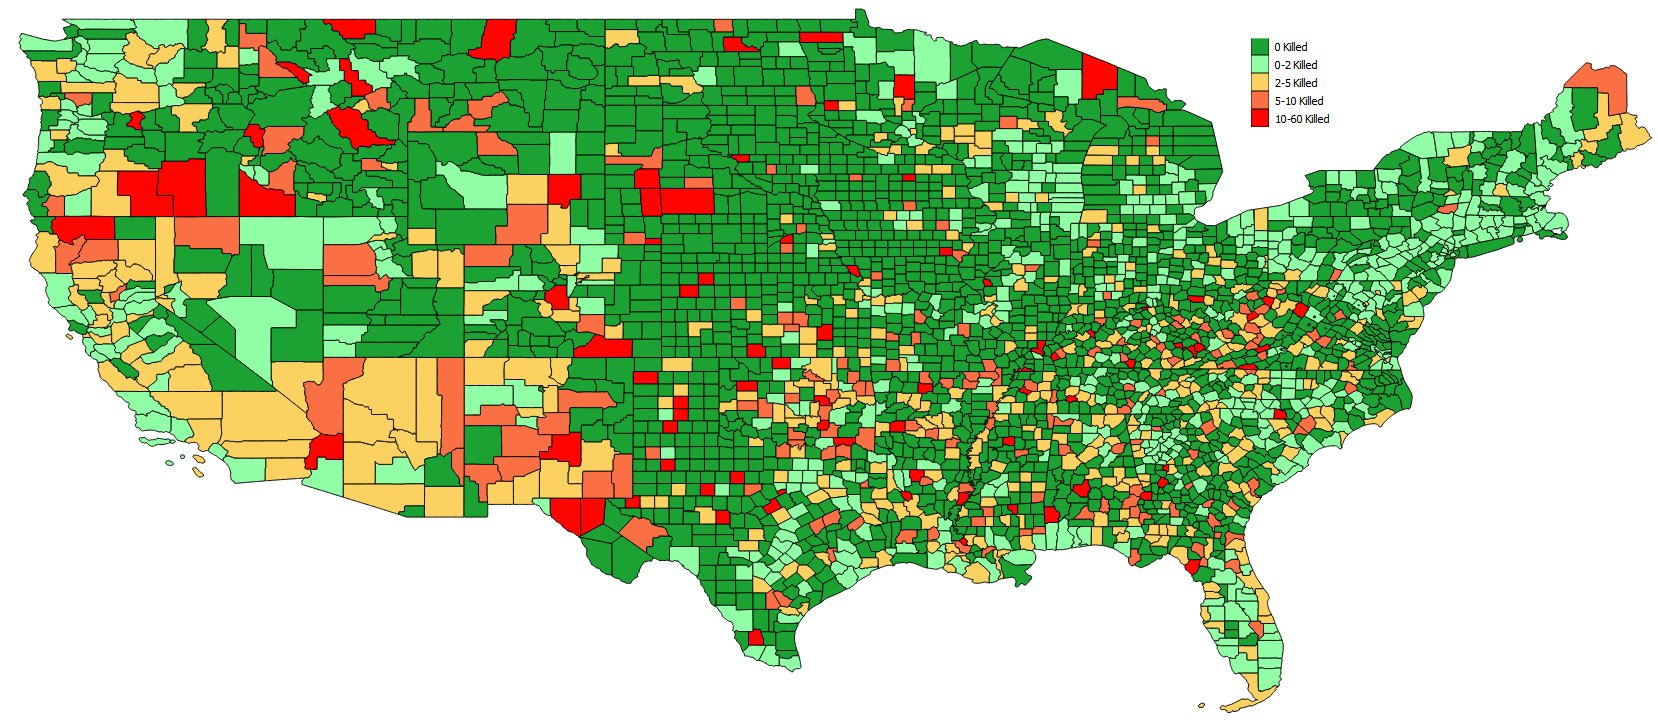
\includegraphics[width=1.0\textwidth]{images/figure1.jpg}
\caption{U.S. county-level map of residents killed by police, 2013-Oct 2017.  Data from Census and MappingPoliceViolence.org}
\end{figure}

\begin{figure}
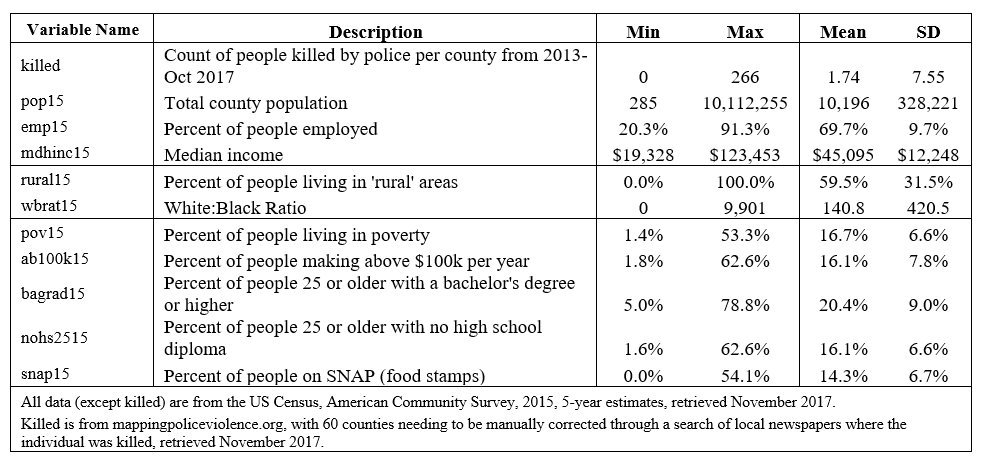
\includegraphics[width=1.0\textwidth]{images/table1.jpg}
\caption{All variables used in this study.}
\end{figure}

\begin{figure}
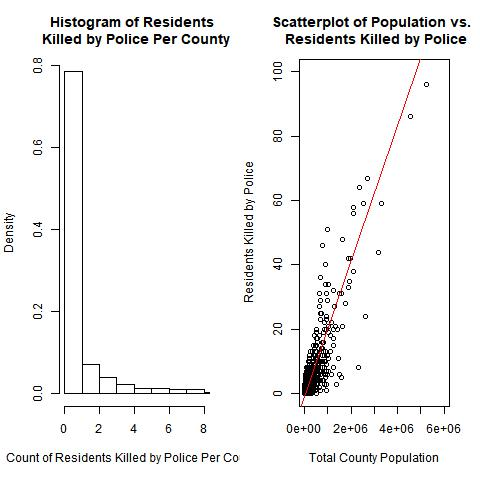
\includegraphics[width=1.0\textwidth]{images/figure4.jpg}
\caption{Left: Histogram of the number of county residents killed by police.  This histogram shows a maximum of eight per county killed by police, while the actual maximum is 266.  However, there are only 120 observations where this value is above 8.  This view gives a better depiction of the data.  Right: Scatterplot of the total county population versus the total killed by police in that county.  The red line is a regression prediction line for these two variables.}
\end{figure}

\begin{figure}
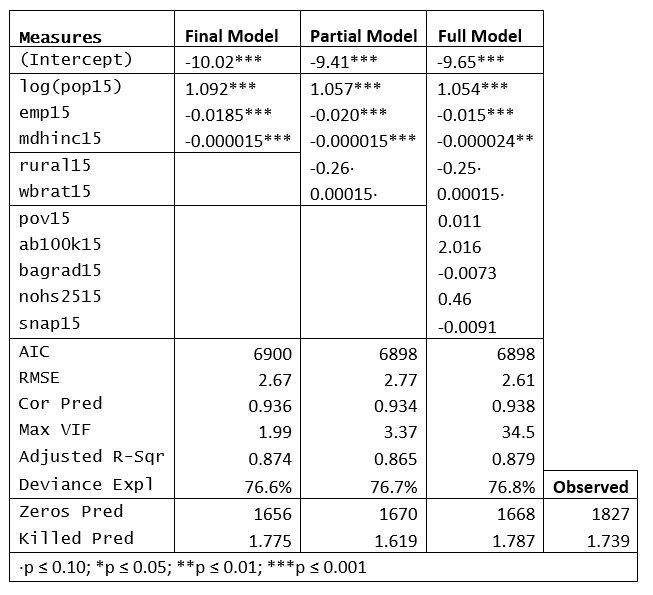
\includegraphics[width=1.0\textwidth]{images/table2.jpg}
\caption{Regression and diagnostic results from all three models.  "Zeros Pred" are the number of counties where no person is predicted to be killed by police, calculated not at exact zero, but any value less than 0.5.  "Killed Pred" is the mean number of predicted people killed by police in each county.}
\end{figure}

\begin{figure}
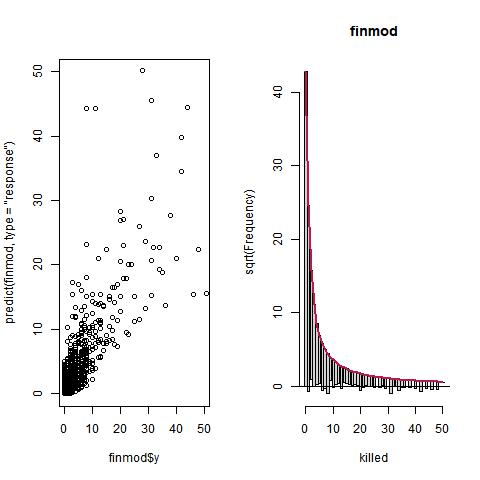
\includegraphics[width=1.0\textwidth]{images/figure2.jpg}
\caption{Left: Scatterplot of predicted versus observed counts of residents killed by police per county. Right: Rootogram--fit of the final regression model: negative binomial with three independent variables (log of population, employment and median income).  The red line can be interpreted as the observed values.  Bars that are hanging below the zero-line are underfit for that bin, and those above the line are overfit for that bin.}
\end{figure}

\begin{figure}
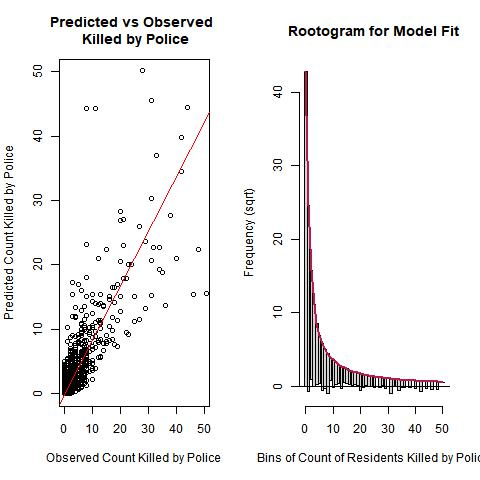
\includegraphics[width=1.0\textwidth]{images/figure3.jpg}
\caption{Regression diagnostics plots for the final model with three independent variables: population (log), employment and median income. Top: Residuals versus fitted and index.  Bottom: Quantile residuals and QQ Plot. }
\end{figure}


\section{Conclusion}
\bibliographystyle{ACM-Reference-Format}
\bibliography{report} 

\end{document}
